\documentclass[12pt,a4paper]{article}

\usepackage[utf8]{inputenc}
\usepackage[ngerman]{babel}
\usepackage[T1]{fontenc}
\usepackage{amsmath}
\usepackage{amsfonts}
\usepackage{amssymb}
\usepackage{graphicx}
\usepackage[left=2cm,right=2cm,top=2cm,bottom=2cm]{geometry}
\usepackage{multicol}
\usepackage{booktabs}
\usepackage[hidelinks]{hyperref}
\usepackage{tikz}
\usepackage{pgfplots}
\usepackage{blindtext}
\usepackage{array}
\usepackage{multirow}
\usepackage{bigdelim}
\usepackage{colortbl}
\usepackage{fancyhdr} 
\usepackage{tabularx}
\usepackage{xcolor}
\usepackage{color}
\usetikzlibrary{decorations.text}
\usetikzlibrary{tikzmark}
\pagestyle{fancy} 
	\fancyhf{} 
	\fancyhead[L]{
\includegraphics[scale=0.05]{Bilder/dhbw.png}} 
	\fancyhead[C]{\slshape Formale Sprachen und Automaten} 
	\fancyhead[R]{\slshape LaTeX Version}
	\fancyfoot[C]{\thepage}
\usepackage{helvet}
\renewcommand{\familydefault}{\sfdefault}

\title{Formale Sprachen und Automaten}
\author{\slshape Robin Rausch, Florian Maslowski}
\date{\slshape \today}
\begin{document}
\pagenumbering{Roman}
\maketitle
\tableofcontents
\newpage
\pagenumbering{arabic}
\section{Grundlagen}
\subsection{Alphabet}
Ein Alphabet $\varSigma$ ist eine nicht-leere Menge von Symbolen(Zeichen, Buchstaben).
Beispiel: $\varSigma_{ab} = { a, b }$

\subsection{Wort}
Ein Wort $w$ über dem Alphabet $\varSigma$(Sigma) ist eine endliche Folge von Symbolen aus $\varSigma$. Das Wort $w = abaabab$ wurde beispielsweise aus dem Alphabet $\varSigma_{ab}$ gebildet.\newline
Die Länge eines Wortes kann durch Betragsstriche angegeben werden. Beispiel: $|w| = 7$\newline
Ebenso kann man die Anzahl bestimmter Symbole in einem Wort bestimmen: $|w|_b = 3$\newline
Ein einzelnes Zeichen kann durch eckige Klammern angegeben werden: $w[2] = b$\newline
Wörter können bliebig konkateniert werden(hintereinanderschreiben ohne abstand): $w_1w_2 = abbabaab$ mit $w_1 = abba$ und $w_2 = baab$.\newline
Wörter dürfen auch potenziert werden: $w^3 = abaabababaabababaabab = www$\newline
Das leere Wort lautet $\varepsilon$.

\subsection{Formale Sprachen}
Eine formale Sprache $L$ über einem Alphabet $\varSigma$ ist eine Menge von Wörtern aus $\varSigma^*: L \subseteq \varSigma^*$. Eine Sprache kann sowohl endlich als auch unendlich sein.\newline
Beispiel: $L_1 = \{w \in \varSigma_{bin}^* |$ $|w| \geqslant 2 \wedge w[|w| - 1] = 1\}$ ist die Menge aller Binärwörter, an deren vorletzter Stelle 1 steht.\newline
Das Produkt zweier formaler Sprachen: $L_1 \cdot L_2 = \{abac, abcb, bcac, bccb\}$ mit $L_1 = \{ab, bc\}$ und $L_2 = \{ ac, cb\}$.\newline
Sprachen können ebenfalls potenziert werden: $L^2 = \{ab, ba\} \cdot \{ab, ba\} = \{ abab, abba, baab, baba\}$

\subsection{Kleene Stern}
Für ein Alphabet $\varSigma$ und eine formale Sprache $L \subseteq \varSigma^*$ ist der Operator Kleene Stern wie folgt definiert: $L^* = \underset{n \in \mathbb{N}}{\bigcup} L^n$.\newline \newline
Beispiel: Sei $L_1 = \{ ab, ba\}$, dann $L^* = \{\varepsilon, ab, ba, abab, abba, baab, baba, ababab, ...\}$.

\section{Reguläre Sprachen und endliche Ausdrücke}
\subsection{Reguläre Ausdrücke}
Ein regulärer Ausdruck über $\varSigma$ beschreibt eine formale Sprache.\newline
Die Menge aller regulären Ausdrücke über $\varSigma$ ist eine formale Sprache.\newline\newline
Beispiel: Sprache aller Wörter über $\varSigma_{abc}$, die nur aus genau zwei Symbolen bestehen:\newline
Ausdruck: $r_1 = (a + b + c)(a + b + c)$\newline
Sprache: $\mathcal{L}(r_1) = \{ w \in \varSigma_{abc}^*$ | $|w| = 2\}$\newpage
\noindent Operatoren:
\begin{center}
	\begin{figure}[!h]
		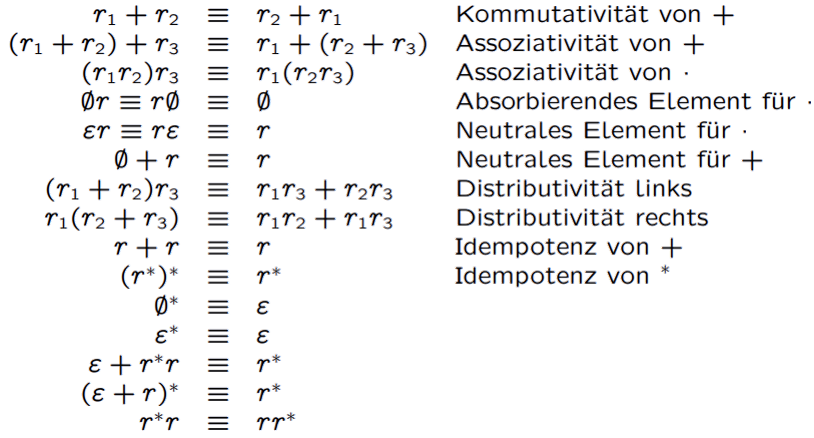
\includegraphics[width=\textwidth]{Bilder/RegulaereAusdruecke_Operatoren.PNG}
	\end{figure}
\end{center}
Nicht alle Operatoren sind für alle Typen zulässig:
\begin{center}
	\begin{figure}[!h]
		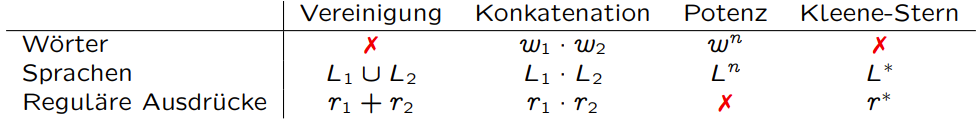
\includegraphics[width=\textwidth]{Bilder/Zulaessige_Operatoren.PNG}
	\end{figure}
\end{center}

\subsection{Endliche Automaten}
Endliche Automaten sind eine andere Darstellung einer regulären Sprache. Endliche Ausdrücke lassen sich in Reguläre Ausdrücke umformen. Genauso auch anders herum.\newline
Endliche Automaten erkennen regulären Sprachen. Endliche Ausdrücke lassen sich in Reguläre Ausdrücke umformen. Genauso auch anders herum.\newline
Endliche Automaten lassen sich sowohl deterministisch als auch nicht-deterministisch darstellen.

\subsubsection{Deterministische endliche Automaten(DEA)}
Ein DEA hat endlich viele Zustände. Jeder mögliche Übergang muss hierbei behandelt werden können. D.h. für das Alphabet $\varSigma_{ab}$ muss von jedem Zustand sowohl ein $a$, als auch ein $b$ Übergang gegeben sein. Der Automat beginnt im Startzustand und muss im Endzustand enden. Wenn der Automat sich in einem Nicht-Endzustand befindet, befindet sich das Wort nicht in der Sprache, welche vom Automaten abgebildet wird.\newline
Ein DEA hat endlich viele Zustände. Jeder mögliche Übergang muss hierbei behandelt werden können. D.h. für das Alphabet $\varSigma_{ab}$ muss von jedem Zustand sowohl ein $a$, als auch ein $b$ Übergang gegeben sein. Er terminiert wenn das Wort zu ende und Endzustand erreicht ist.
\noindent Der DEA lässt sich durch folgendes 5-Tupel darstellen:\newline
$\mathcal{A} = (Q, \varSigma, \delta, q_0, F)$ mit den Komponenten:\newline
$Q$ ist eine endliche Menge von Zuständen\newline
$\varSigma$ ist ein endliches Alphabet\newline
$\delta: Q \times \varSigma \rightarrow Q$ ist die Übergangsfunktion\newline
$q_0 \in Q$ ist der Startzustand\newline
$F \subseteq Q$ ist die Menge der Endzustände\newline
\newline
Beispiel:\newline
\begin{center}
	\begin{figure}[!h]
		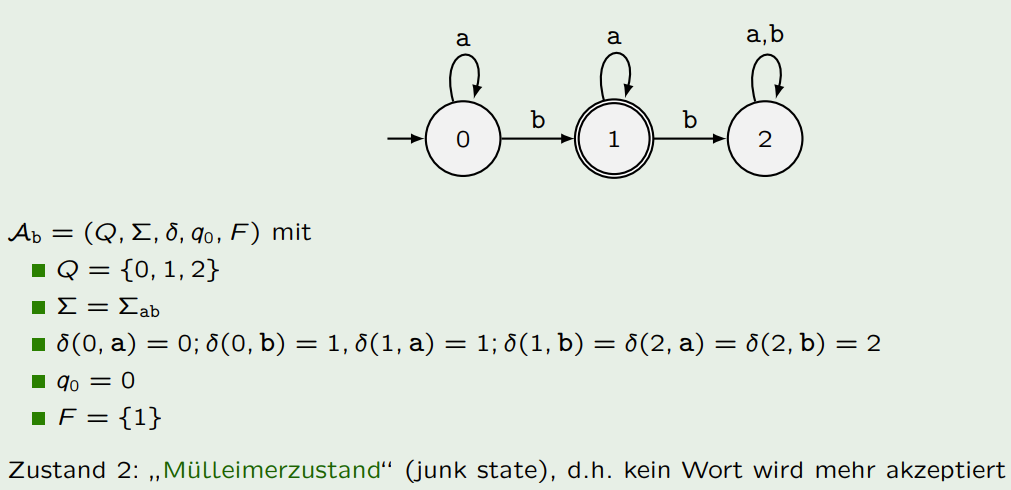
\includegraphics[width=\textwidth]{Bilder/DEA_Beispiel.PNG}
	\end{figure}
\end{center}

\subsubsection{Nicht-deterministische endliche Automaten(NEA)}
Ein NEA hat endlich viele Zustände. Nicht jeder mögliche Übergang muss hierbei behandelt werden. D.h. für das Alphabet $\varSigma_{ab}$ reicht es, nur den $a$-Übergang, bzw. nur den $b$-Übergang zu besitzen. Der Automat beginnt im Startzustand und muss im Endzustand enden. Wenn der Automat sich in einem Nicht-Endzustand befindet, befindet sich das Wort nicht in der Sprache, welche vom Automaten abgebildet wird. Zudem gibt es $\varepsilon$-Übergänge, diese können jederzeit verwendet werden ohne ein Eingabesymbol.\newline
\noindent Der NEA lässt sich durch folgendes 5-Tupel darstellen:\newline
$\mathcal{A} = (Q, \varSigma, \Delta , q_0, F)$ mit den Komponenten:\newline
$Q$ ist eine endliche Menge von Zuständen\newline
$\varSigma$ ist ein endliches Alphabet\newline
$\Delta$ ist eine Relation über $Q \times (\varSigma \cup \{\varepsilon\}) \times Q$\newline
$q_0 \in Q$ ist der Startzustand\newline
$F \subseteq Q$ ist die Menge der Endzustände\newline
\newline
Beispiel:\newline
\begin{center}
	\begin{figure}[!h]
		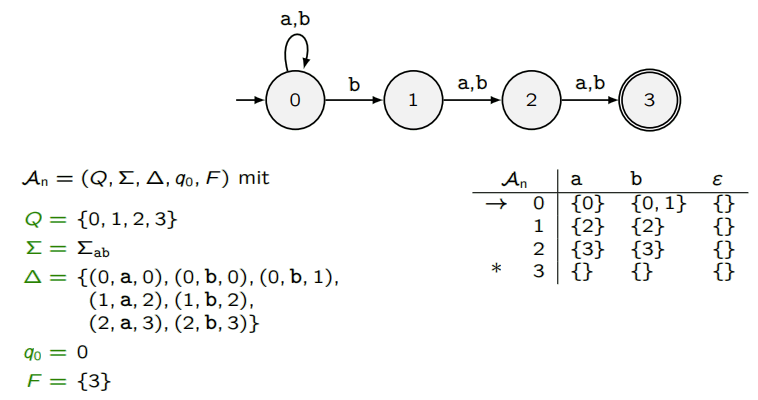
\includegraphics[width=\textwidth]{Bilder/NEA_Beispiel.png}
	\end{figure}
\end{center}

\subsubsection{Endliche Automaten und reguläre Ausdrücke}
Man kann NEA und RA zusammenführen zu einem Automaten:\newline
\begin{center}
	\begin{figure}[!h]
		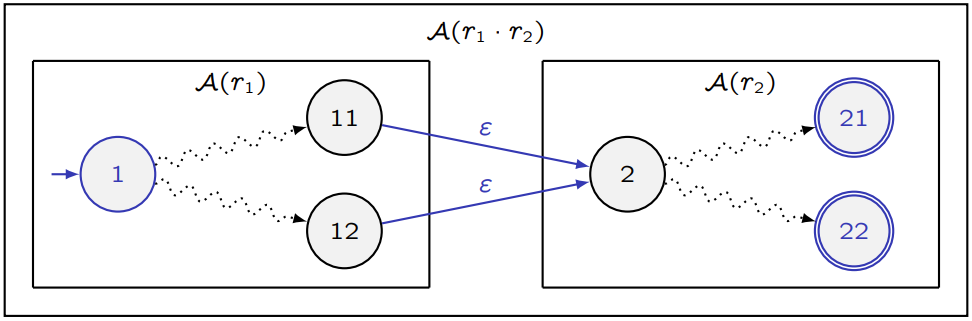
\includegraphics[width=\textwidth]{Bilder/Konkatenation.png}
	\end{figure}
\end{center}
\begin{minipage}[c]{0.49\textwidth}
	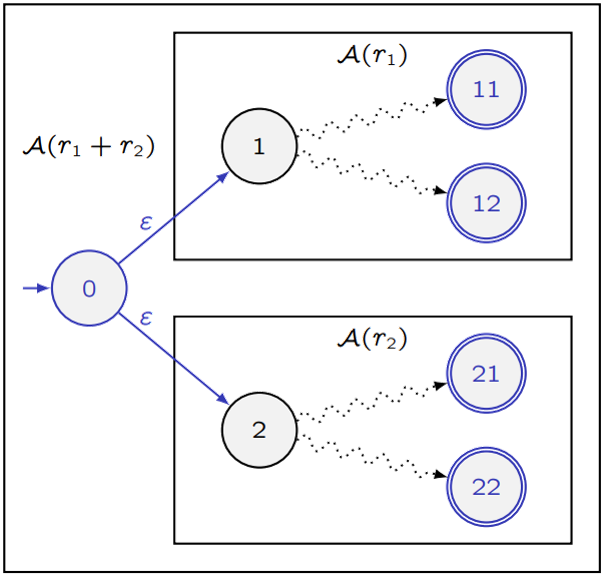
\includegraphics[width=\textwidth]{Bilder/Vereinigung.png}
\end{minipage}
\begin{minipage}[c]{0.49\textwidth}
	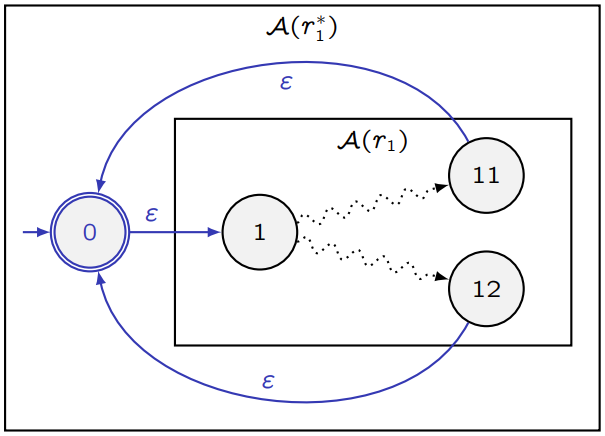
\includegraphics[width=\textwidth]{Bilder/KleeneStern.png}
\end{minipage}

\subsubsection{Transformation DEA zu RA}
Um einen DEA zu einem RA umzuformen müssen zuerst die Gleichungen der jeweiligen Zustände aufgestellt und vereinfacht werden:\newline
\begin{center}
	\begin{figure}[!h]
		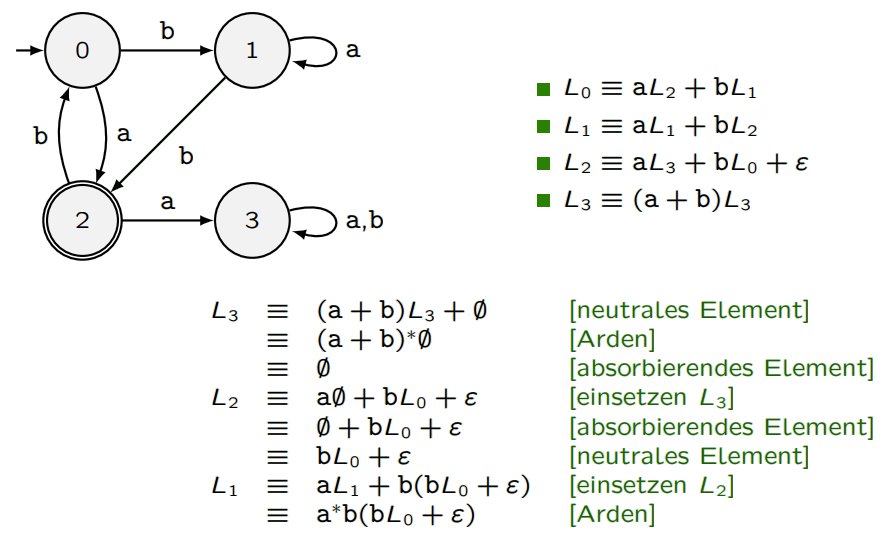
\includegraphics[width=\textwidth]{Bilder/DEAzuRA1.png}
	\end{figure}
\end{center}
Folglich kann man die gekürzten Gleichungen in einander einsetzen um bis zum Anfangszustand zu kommen:\newline
\begin{center}
	\begin{figure}[!h]
		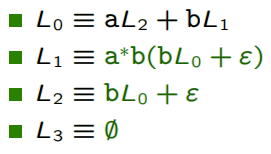
\includegraphics[]{Bilder/DEAzuRA2.png}
	\end{figure}
\end{center}
Da $L_2$ der Endzustand ist, bekommt die Gleichung $\varepsilon$ hinzuaddiert!\newline
Der vereinfachte Anfangszustand $L_0$ ist dann der RA zum zugehörigen DEA:\newline
\begin{center}
	\begin{figure}[!h]
		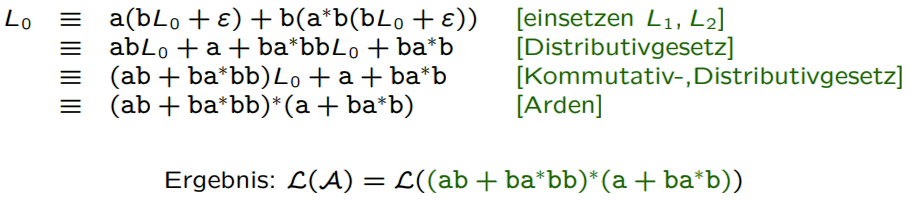
\includegraphics[width=\textwidth]{Bilder/DEAzuRA3.png}
	\end{figure}
\end{center}

\subsubsection{Minimierung}

\subsection{Nicht-reguläre Sprachen und das Pumping-Lemma}

\subsection{Eigenschaften regulärer Sprachen}

\section{Chomsky Grammatiken und kontextfreie Sprachen}
	Gramatiken erzeugen formale Sprachen dar.\\
	G=($N, \sum , P, S$) mit:\\
	\begin{description}
		\item[N] Nichtterminalsymbole. Diese können für Regeln verwendet werden, aber dürfen nicht selbst im abgeleiteten Wort stehen.
		\item[P] Ableitungsregeln. Bsp.: P=$\{ S \rightarrow Aa | \varepsilon , A \rightarrow a \} $ 
		\item[S] Startsymbol (ist nichtterminel)
	\end{description}

	\subsection{Typ0 unbeschränkt}
    \subsection{Typ1 Monoton}
    $\alpha \rightarrow \beta$ mit $| \alpha | \leq  | \beta |$ und Ausnahme $S \rightarrow \varepsilon$, wenn S auf keiner rechten Seite ist.
    \subsection{Typ2 Kontextfreie}
	A $\rightarrow \beta$ mit A $\in$ N und $\beta \in V$* 
    \subsection{Typ3 rechtsregulär/-linear}
	A $\rightarrow$ cB mit A $\in$ N; B $\in$ N $\cup$ $\{ \varepsilon \}$; c $\in \sum \cup \{ \varepsilon \}$
	\subsection{Cocke-Younger-Kasami(CYK)-Algorythmus}
	Entscheidet Wortproblem für kontextfreie Grammatiken in CNF. Bsp.:\\
	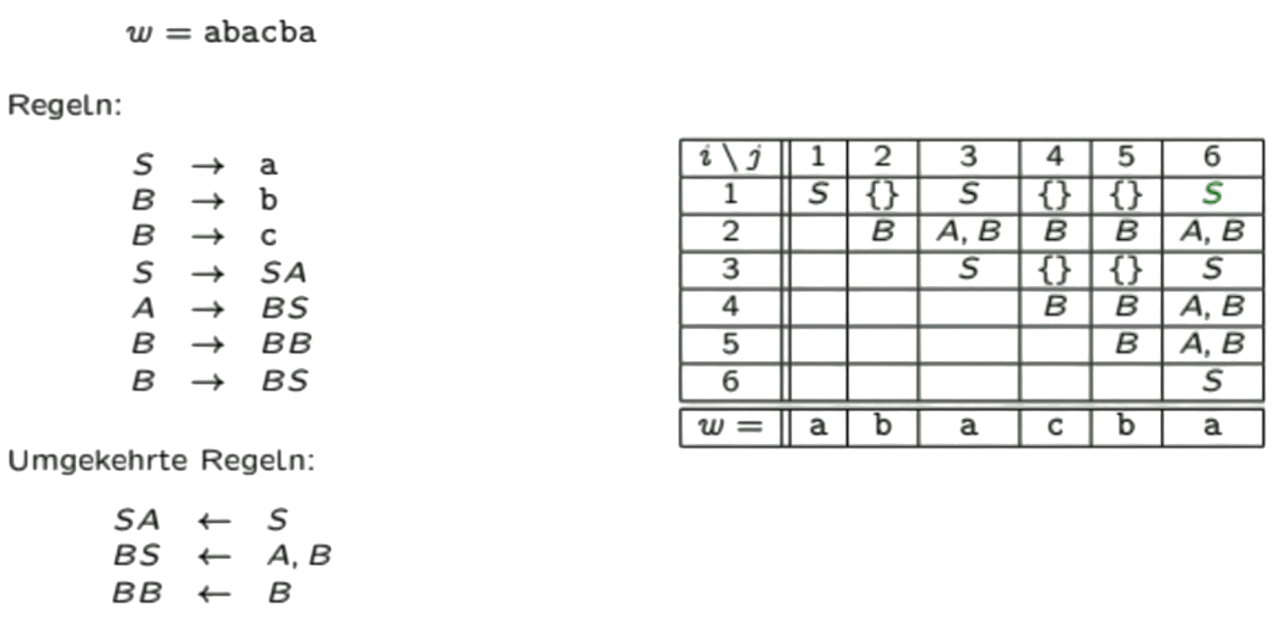
\includegraphics[scale=0.3]{Bilder/cyk-Algo.png}
	\begin{enumerate}
		\item Wort unter Tabelle schreiben 
		\item Umgekehrte Regeln bilden (optional)
		\item Herleitungen in Tabellen-Diagonale eintragen
		\item Herleitungen der Teilwörter als Menge eintragen (alle Möglichkeiten)
	\end{enumerate}
	\subsection{Chomskynormalform CNF}
	Zur Entscheidung des Wortproblems. Nur Regeln mit Syntax: \\
	1. $A \rightarrow BC$ oder 2. $A \rightarrow a$ mit $A,B,C \in Nichtterminalsymbole \; \wedge \; a \in Terminalsymbole$ und $S \rightarrow \epsilon$, wenn S auf keiner Rechten Seite ist.\\
	\textbf{Vorgehen:}
	\begin{enumerate}
		\item Epsilon-Regeln entfernen
		\begin{enumerate}
			\item Erstelle Liste L mit $A\rightarrow \epsilon$-Regeln und allen Regeln, die auf Nichtterminalsymbole in L zeigen.
			\item Ergänze rechte Seite der Regeln mit sich selbst mit eingesetztem $\epsilon$ für Nichtterminalsymbole $\in$ L
			\item Wenn $S \in L$ füge Regel $S_0 \rightarrow S | \epsilon$ ein
		\end{enumerate}
		\item Kettenregel entfernen
		\begin{enumerate}
			\item Erstelle Listen für Kettenregeln ausgehend von jeweiligen Nichtterminalen
			\item Ergänze Regeln mit allen Kettenregeln
			\item Regeln kürzen
		\end{enumerate}
		\item überflüssige Symbole entfernen
		\item Einzelne Nichtterminalsymbole auf rechter Seite ersetzen 
		\item Rechte Seite mit Hilfssymbolen kürzen
	\end{enumerate}

\section{Turing Maschine}
	Automaten mit endlosem Einleseband.\\
	Terminiert wenn Endzustand erreicht und Einleseband nicht verschiebbar ist.\\
	M=(Q, $\sum, \Gamma , \Delta , q_0$, F) mit:\\
	\begin{description}
		\item[$\Gamma$] Vereinigung aus mindestens Blank-Symbol und Terminalsymbole: $\Gamma \supseteq \sum \cup \{ \square \} $
		\item[$\Delta$] Übergangsrelationen Syntax: IST-Zustand IST-Inhalt Neuer-Inhalt Verschiebung Neuer-Zustand Bsp.: $0 \left( \begin{array}{c} a \\ \square \end{array}\right) \left( \begin{array}{c} a \\ a \end{array}\right) \left( \begin{array}{c} r \\ l \end{array} \right) 1$
		\item[F] Endzustände
	\end{description}

\section{Entscheidbarkeit}
	\subsection{Entscheidbar}

	\subsection{Unentscheidbar}

	\subsection{Semi-entscheidbar}

\section{Berechenbarkeit}

\section{Komplexität}

\end{document}